\documentclass[a4paper,10pt, english]{article}

\usepackage{amssymb}
\usepackage{amsmath}
\usepackage{enumitem}
\usepackage{graphicx}
\usepackage{subfig}
\usepackage{amsthm}




\newcommand{\D}{\displaystyle}

\newtheorem{theo}{Theorem}[section]
\newtheorem{dfn}{Definition}[section]
\newcommand{\R}{\mathbb{R}}
\newtheorem{prop}[theo]{Proposition}



















\begin{document}


\title{Optimal and feedback decentrilized control for Cucker Smale system}
\author{M. Kryven, M. Caponigro, A. Borzi}
\maketitle








\section{Introduction}
The aim of this work is to design a decentralized optimal control strategy for the Cucker-Smale system to steer the system to consensus while maintaining the spatial connectivity of the initial interaction graph.

Consider the Cucker-Smale system
\begin{align}
\begin{cases}
\D
\dot{x_i} = v_i,\\
\dot{v_i} = \frac{1}{N}\sum_{j=1}^{N}a(\|x_i - x_j\|)(v_j - v_i) + u_i, \\
x(0) = x_0,
v(0) = v_0.
\end{cases}
\label{csm}
\end{align}
where $i =1, \dots, N$, $N$ is the number of  $d$-dimensional agents, a pair $(x_i, v_i)\in \mathbb{R}^{2d}$, represents the position and velocity of every agent, $u_i$ is an external controller. This kind of model has been introduced by Cucker and Smale in \cite{cs1} - \cite{cs2} for specific choices of the interaction function $a$ as
\begin{equation}
a(r) = \frac{1}{(1 + r^2)^\delta} \qquad \mbox{for every}\quad \delta \in [0, +\infty],
\label{a}
\end{equation}
this function defines the natural interaction force between agents. The unconditional consensus emergence largely depends on the strength of the force. In \cite{cs2} a result was presented related to the parameter $\delta$ in (\ref{a}); it asserts that for $\delta \leq 1/2$, the system tends asymptotically to consensus, independent of its initial configuration. For $\delta > 1/2$, consensus emergence will depend on the cohesion of the initial setting. A precise characterization of this situation was obtained in \cite{theorem11} where a sufficient condition depending on the initial configuration and the parameter $\delta$ is provided. To state this condition let us define a symmetric bilinear form $B$ on $\mathbb{R}^{N\times d} \times  \mathbb{R}^{N\times d}$ by
\begin{equation}
B(u, v) = \frac{1}{2N^2}\sum_{i, j \in \mathcal{I}} \langle u_i - u_j, v_i - v_j  \rangle,
\label{b}
\end{equation}
where $\langle . \rangle$ denotes a scalar product in $\mathbb{R}^d$.
\begin{theo}
Let $(x_0, v_0) \in \mathbb{R}^{N\times d} \times  \mathbb{R}^{N\times d}$ satisfy
\begin{equation}
E(x_0, v_0):=\sqrt{B(v_0, v_0)} - \int_{\sqrt{B(x_0, x_0)}}^{\infty} a(\sqrt{2N}r)dr \leq 0.
\label{cq}
\end{equation}
Then the solution of uncontrolled system (\ref{csm}) with initial data $(x_0, v_0)$  tends to consensus.
\end{theo}

There have been developed many analytical feedback control strategies  to steer the system (\ref{csm}) to consensus. In particular in \cite{cftp} it is shown that with a controller 
of the form
$$
u_i = \bar{v} - v_i,
$$
consensus emergence can be guaranteed for any configuration and values of $\delta$. A natural drawback of such a controller relates to the fact that is is always active, and it involves the whole system at every
instant of time. Later on,  in \cite{bfk} a decentralized control setting  was studied \--- a local feedback depending on a metrical neighbourhood of the agents. The neighbours consist of all agents 
the distance to which is less than a specified number $R>0$
\begin{equation}
u_i = \bar{v}_i - v_i,
\label{bfk}
\end{equation}
where $\bar{v}_i$ is an approximated mean velocity vector in the neighbourhood of radius $R$ instead of the true mean velocity of the whole group $\bar{v}$. This control guarantees the consensus emergence under certain initial conditions.




Let us define a distance dependent dynamic graph for the interactions between agents.
\begin{dfn}
We call $\mathcal{G}(t) =  (\mathcal{V}, \mathcal{E}(t) )$ a dynamic graph consisting of a set of vertices $\mathcal{V} = \{1, \dots,  N\}$ indexed by the set of agents and a time varying set of links 
$\mathcal{E}(t) = \{(i, j)|i, j \in \mathcal{V}\}$ such that, for any $R>0$
$$
\mbox{if}\quad 0<\|x_i(t) - x_j(t)\| \leq R \quad\mbox{then},\quad (i, j)\in \mathcal{E}(t).
$$
\end{dfn}
And let us denote $\mathcal{N}_i(t) = \{j|(i, j)\in\mathcal{E}(t)\}$ the neighbourhood of agent i.
Let us also denote an agent along with its neighbours as a set $\bar{\mathcal{N}}_i(t) = \mathcal{N}_i(t)\bigcup \{i\}$.
In \cite{jfwpc} a distributed control law, based on potential fields, that achieve velocity alignment and maintain the existing links in the network was developed 
\begin{equation}
u_i = \bar{v}_i - v_i - \sum_{j \in \mathcal{N}_i(t)}\nabla_{x_i}V(\|x_i - x_j\|).
\label{controljad}
\end{equation}
where $\bar{v}_i = \sum_{j \in \mathcal{N}_i(t)} v_j$, and $V$ is a potential function  to maintain the connectivity of the initial interaction graph $\mathcal{G}(0)$ 
\begin{equation}
 V(r) = \frac{1}{r^2} + \frac{1}{R^2 - r^2}, \qquad 0 < r < R.
\label{potential}
\end{equation}
This potential not only allows for maintaining links in the network but also for avoiding collisions among the agents. 

In this paper we would like to design decentralized feedback and optimal control strategies which aim to steer the system to consensus as well as maintaining the connectivity.





\newpage
\section{Feedback control that guarantees connectivity for the Cucker-Smale system}
Consider the feedback control for the Cucker-Smale system 

\begin{equation}
u_i(t) = \sum_{\mathcal{N_{i}(t)}}W(\|x_i(t) - x_j(t)\|) \nabla_{x_i} \frac{d}{dt}\|x_j(t) - x_i(t)\|,
\label{myhc}
\end{equation}
where $W$ is a potential of the form
\begin{equation}
 W(r) = \frac{(R/2)^4}{((r - R/2)^2  - R^2/4)^2} + 1.
\label{potentialw}
\end{equation}
This potential has almost the same effect as (\ref{potential}) it increases the binding force between agents as they are about to break the network connectivity as well as rules out collisions with the difference that it acts directly on velocity alignment rather than spatial distance between agents and still guarantees the connectivity of the network. Note, that it smoothly decays Figure \ref{potentialwplot} as the distance between agents deviates from the safe one which is $R/2$, if $\|x_i - x_j\| = R/2$ the control completely switches of since the agents $i$ and $j$ are at a safe distance from breaking the connectivity or colliding, 
as soon as  $\|x_i - x_j\| > R/2$ or $\|x_i - x_j\| < R/2$ the control smoothly increases its force and becomes unbounded as $\|x_i - x_j\|$ approaches $0$ or $R$ to prevent the network connectivity breach or collisions respectively. 
\begin{figure}[ht]
 \centering
 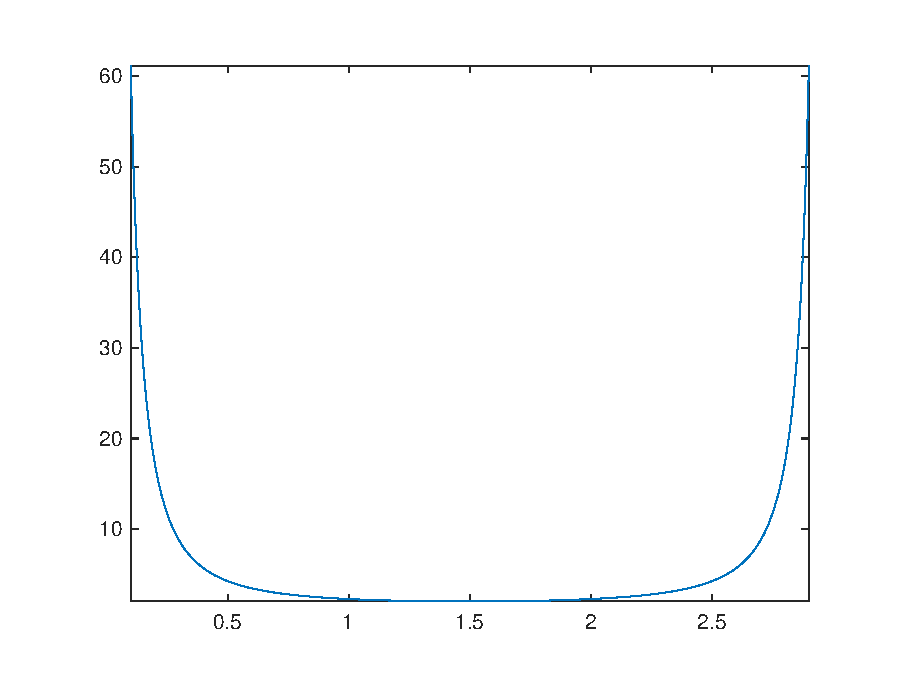
\includegraphics[scale=0.5]{figures/potentialwplot.eps}
 \caption{$W(t)$}
 \label{potentialwplot}
\end{figure}
Control (\ref{myhc}) is virtually control (\ref{bfk})  scaled by a force factor $W$, since $\frac{d}{dt}\|x_j(t) - x_i(t)\| = 2(v_j - v_i)$. It is more natural than (\ref{controljad}) because the physical 
units remain to be that of velocity rather than spatial ones. With such control we can use the same argument as in \cite{jfwpc} with potential (\ref{potential}) replaced by (\ref{potentialw})  to verify that for the system (\ref{csm}), (\ref{myhc})  
for any pair of switching times $t_p < t_q$ the switching topology satisfies $\mathcal{G}(t_p) \subset \mathcal{G}(t_q)$ what implies that the connectivity of the network does not decrease with time.
And according to Theorem 3.3 from \cite{jfwpc} all agent velocities become asymptotically the same and collisions among agents are avoided. 






\section{The decentralized MPC strategy}
  We would like to design a decentralized control strategy with the same aims as (\ref{controljad}) and (\ref{myhc}) such that it is optimal in some sense. For this we consider minimizing a functional 
 
  \begin{equation}
  \min_{x, v} J(x, v) = \int_{0}^{T}\frac{1}{N}\sum_{i=1}^{N}\|v_i(t) - \bar{v}(t)\|^2 dt + \frac{1}{N}\sum_{i=1}^{N}\|v_i(T) - \bar{v}(T)\|^2,
 \label{j}
 \end{equation}
 subject to (\ref{csm}). The first term stands for the agents' velocity alignment throughout the evolution and the second one accentuates the consensus emergence at the terminal configuration. 
 
 To introduce decentralization we decompose the state domain in sub-domains $\bar{\mathcal{N}}_p(t)$ for every $p\in \mathcal{I}$ where an optimal control problem is solved independently to obtain the suitable decentralized control for agent $p$. Such decentralization has already been utilized for first order systems in \cite{jdccms}.
 The algorithm adopts the model predictive control approach by partitioning the time interval $[0, T]$ into $m$ time windows where subsequently solving an optimal control problem for each agent $p$.
 
 
 The general idea of model predictive control is that future control inputs and future state are predicted using the system model and optimized at regular intervals. For
 the time interval $[0, T]$ where the evolution of system (\ref{csm}) is considered. 
 The time interval is partitioned into $m\in \mathbb{N}$ uniform time windows $[T_{l-1}, T_{l}]$, $l = 1, \dots, m$, $T_0 = 0, \dots, T_m = T$  of length  $\Delta T = T/m$. The genereal MPC strategy starts at zero time and solves the open-loop control problem defined in the interval $[T_0, T_1]$. Then, with response  resulting at time $T_1$ we have the initial condition for the subsequent optimization problem defined in the interval $[T_1, T_2]$. This procedure is repeated by receding the time horizon until the last window is reached. We implement the MPC scheme where the time horizon used to evaluate the control coincides with the time horizon where the control is used.
 
 
   The decentralization comes with state domain decomposition on each time window $[T_{l-1}, T_{l}]$, $l = 1, \dots, m$  of the MPC scheme where for each agent $p$, $p = 1, \dots, N$ we solve an optimal control problem for a state domain $\bar{\mathcal{N}}_p(T_{l-1})$ where the information is exchanged only between agent $p$ and its neighbours and not between the neighbours themselves
   \begin{equation}
    \min_{x, v} J_p(x, v) = B_p(v(T_l)) + \int_{T_{l-1}}^{T_l}\sum_{j\in \mathcal{N}_p(T_{l-1})} U(\|x_p(t) - x_j(t)\|),
   \label{jp}
   \end{equation}
   subject to 
   \begin{align}
   \begin{cases}
   \D
   \dot{x_i} = v_i,\\
   \dot{v_p} = \frac{1}{N_p}\sum_{j\in \mathcal{N}_p(T_{l-1})}a(\|x_i - x_j\|)(v_j - v_i) + u_p, \\
   \dot{v_i} = \frac{1}{N_p}\sum_{j\in \mathcal{N}_p(T_{l-1})}a(\|x_i - x_j\|)(v_j - v_i),\\
   \end{cases}
   \label{csmp}
   \end{align}
  for $i\in\mathcal{N}_p(T_{l-1})$, where $N_p:= \# \bar{\mathcal{N}}_p(T_{l-1})$, with initial conditions $(x(T_{l-1}), v(T_{l-1}))$ taken as endpoints form the solution on the previous time window $l-1$,
  the functional $B_p(v(t))$ has the following form 
  \begin{equation}
  B_p(v) = \frac{1}{N_p}\sum_{j \in \mathcal{N}_p(t)} \| v_p - v_j \|^2,
  \label{bp}
  \end{equation}
  it is chosen so that it makes the agent  $p$ to align its velocity to its neighbours and 
  $U$ is a potential that measures the relative distance between agents which we would like to minimize to maintain the network connectivity
    \begin{equation}
    U(r) = (R/N- r)^2, \qquad 0 < r.
    \label{potentialbar}
    \end{equation}
    The idea of this potential is to increase the force with which the agents are pulled together as number of the agents increases, which would provide the increased connectivity of the network at the terminal configuration. Note, that we can not use the same potential as in (\ref{potential}) or (\ref{potentialw}) because the functional $J$ will not be coercive.
  
 Given OPC (\ref{jp})-(\ref{csmp}), at each time window $l$ for each agent $p$ we obtain a suitable decentralized control $u_p(\mathcal{N}_p(T_l))$ which only depends on its neighbours in the time window $l$.
 For a sufficiently small time window the  neighbourhood of agent $p$ does not change throughout the evolution, therefore we assume it is constant in the time window. 


   The algorithm reads as the following: given the system (\ref{csmp}):
   \begin{enumerate}
   \item Partition time interval $[0, T]$ into time windows $\Delta T$: $0 = T_0, T_1, \dots, T_m = T$.
   \item For each time window  $[T_{l-1}, T_{l}]$, $l = 1, \dots, m$ and for each agent $p$, $p = 1, \dots, N$  solve the OPC (\ref{jp}) - (\ref{csmp}) for the initial conditions $(x(T_{l-1}), v(T_{l-1}))$.
   \item From the solution of (\ref{jp}), (\ref{csmp})  retrieve the  state for the agent $p$ in the time window $l$ $(x_p(t), v_p(t))$ and control $u_p(t)$, $t\in [T_{l-1}, T_{l}]$.
   \item Repeat the steps 2-3 until the solutions for all windows are obtained. 
 \end{enumerate}
 



 
 
 \section{The optimal contro problem and its discretization}
  We represent the optimal control problem  (\ref{jp}), (\ref{csmp}) for agent $p$ on time window $[T_{l-1}, T_{l}]$ in Mayer form.
  
 \begin{align}
 \D
 & \mbox{minimize}\quad  C(X(T)),   \label{compact_cost} \\ 
 & \mbox{subject to} \quad \dot{X} = F(X(t), u(t)), \quad X(0) = X_0, \label{compact_equation}
 \end{align}
where  the control $u \in  L^{\infty}([T_{l-1}, T_{l}], \mathbb{R}^{N_p \times d})$,
the state $X\in H^1([T_{l-1}, T_{l}], \mathbb{R}^{2(N_p \times d)+1})$
in a compact form composed of the position and velocity 
states of (\ref{csmp})   $X(t) = (x(t), v(t), z(t))$, $x(t) = (x_{i_1}(t), \dots, x_{i_{N_p}}(t))$,
 $v(t) = (v_{i_1}(t), \dots, v_{i_{N_p}}(t))$, $\{i_1, \dots, i_{N_p}\} \in \bar{\mathcal{N}}_p(T_l)$, 
 and $z(t)$ is an auxiliary component 
 $$
 z(t) =  \sum_{j\in \mathcal{N}_p(T_{l-1})} U(\|x_p(t) - x_j(t)\|),
 $$
 with the initial condition $z(0) = 0$ and $F(X)$ is the dynamics of the system (\ref{csmp}) in compact form
 $$
 F(X(t), u(t)) =
  \left( 
  \begin{array}{c}
  v(t)\\
   - L_xv(t) + u(t)\\
   z(t)\\
 \end{array} 
 \right), 
 $$
 where $L_x$ is the Laplacian of the $N_p\times N_p$ matrix $(a(\|x_i - x_j\|)/N_p)_{i, j\in\bar{\mathcal{N}}_p(T_{l-1})}$ which depends on $x$, $u(t) = (0, \dots, u_p(t), \dots, 0)$.
 For the functional $C$ to correspond to the problem in its original form it is chosen 
 $$
 C(X(T_l)) = z(T_l) + B(v(T_l), v(T_l)).
 $$
 
  Note, since our problem is autonomous and all time windows are of the same width, without loss of generality
 we can transform the problem on time interval $[0, \Delta T]$. 
 
 
  
  Given the problem (\ref{compact_cost} - \ref{compact_equation}) we discretize it with a third-order Runge-Kutta scheme.  For such scheme, the discrete controls often converge to the continuous solution slower than the discrete state and adjoint variables at the grid points. It  must satisfy an additional condition to achieve third-order accuracy
    for optimal control problems. Here, we utilise a better approximation to the continuous optimal control obtained from a posteriori computation involving the computed discrete state and adjoint variables  developed in \cite{Hager2000}. 
    
  Consider a uniform time mesh and the following time-step size
 \begin{equation}
   h = \frac{\Delta T}{n},
   \label{h}
 \end{equation}
 where $n$ is the total number of discrete time intervals in $[0, \Delta T]$.  The value of $X(t)$ at the discrete time $t_k$ is denoted with
 $$
 X^k = X(t^k), \qquad t^k = kh \quad\mbox{for} \quad k = 1, \dots n.
 $$
 For an $s$-stage Runge-Kutta discretization scheme it is defined by setting the coefficients $a_{ij}$ and
 $b_{i}$, $1\leq i, j\leq s$, such that they satisfy conditions given in \cite{Hager2000}. 
 
 Corresponding to the discretization setting, the optimal control problem (\ref{compact_cost} -  \ref{compact_equation})  attains the following form
 
 \begin{align}
  \D
  & \mbox{minimize}\quad C(X_n), \label{discrete_cost}\\
  & \mbox{subject to} \quad X^{k+1}  = X^k + h\sum_{i=1}^{s}b_iF(y^{ki}, u^{ki}), \qquad X_0 = X(0), \label{discrete_equation_x}\\
  & y^{ki} = X^k + h\sum_{j=1}^{s}a_{ij}F(y^{kj}, u^{kj}),\label{discrete_equation_y}
  \end{align}
 
 for $1\leq i, j\leq s$, and $0\leq k\leq n-1$.
 Where the vectors $y^kj$ and $u^{kj}$ are intermediate state and control variables on the interval $[t^k, t^{k+1}]$. The state uniqueness is guaranteed in \cite{Hager2000}. 
 
 
 

\newpage
\subsection{The gradient evaluation}
Provided the discrete OPC (\ref{discrete_cost} - \ref{discrete_equation_y}) the corresponding  optimality system  is given by

  \begin{align}
   \D
    & X^{k+1}  = X^k + h\sum_{i=1}^{s}b_iF(y^{ki}, u^{ki}), \qquad X_0 = X(0),   \label{os_state_x}\\
 	& y^{ki} = X^k + h\sum_{j=1}^{s}a_{ij}F(y^{kj}, u^{kj}),   \label{os_state_y}\\
 	& p^k = p^{k+1} + h\sum_{i=1}^{s}b_i \chi^{ki}\nabla_x F(y^{ki}, u^{ki}), \qquad p^n = - \nabla_xC(X^n),  \label{os_adjoint_p}\\
 	& \chi^{ki} = p^{k+1} + h\sum_{j=1}^{s} \frac{b_j a_{ji}}{b_i}\chi^{kj}\nabla_x F(y^{kj}, u^{kj}), \label{os_adjoint_psi} 
   \end{align}
where $p^k$ and $\chi^{ki}$ are the adjoint variables.
The first order discrete system (\ref{os_state_x} - \ref{os_adjoint_psi}) provides a convenient way to compute the exact gradient of the discrete cost functional (\ref{discrete_cost})
\begin{equation}
\nabla_{u^{ki}} C(u) = -h b_i \chi^{ki} (\nabla_u F(y^{ki}, u^{ki})), 
\label{discretegradient}
 \end{equation}  
 for $1\leq i, j\leq s$, and $0\leq k\leq n-1$, where the intermediate values for the discrete state and adjoint variables are obtained by first
 solving the discrete state equations (\ref{os_state_x} - \ref{os_state_y}) for $k=0, 1, \dots, n-1$, using the given values for the controls, and then using these computed values for both the state and intermediate variables in (\ref{os_adjoint_p} - \ref{os_adjoint_psi}) when computing the values of the discrete adjoint variable for $k=n-1, n-2, \dots, 0$. Thus the discrete state equation is solved by marching forward from 
 $ k = 0$ while the discrete adjoint equation is solved by marching backwards from $k = n-1$.
 
 The well-posedness of the optimal control problem (\ref{os_state_x} - \ref{os_adjoint_psi}) and error estimates in the discrete approximation are present in \cite{Hager2000}.
 


 \subsection{The NCG scheme}
  For the minimization procedure the nonlinear conjugate gradient  method developed in \cite{hagerzhang} is deployed.
  The reduced functional $C(u):=C(X(u), u)$ is minimized by a sequence
  \begin{equation}
  u^{(k+1)} =   u^{(k)} + \alpha^{(k)} d^{(k)},
  \label{ncgscheme}
   \end{equation}  
  where $\alpha^{(k)}$ is a positive step size and the directions $d^{(k)}$ are generated by the rule
  \begin{equation}
  d^{(k+1)} = - \nabla_u C(u^{(k+1)}) + \beta^{(k)} d^{(k)}, \qquad d^{(0)} = -\nabla_u C(u^{(0)}),
  \label{drct}
  \end{equation}
  \begin{equation}
  \beta^{(k)} = \frac{1}{(d^{(k)})^T y^{(k)}} \left( y^{(k)} - 2d^{(k)}\frac{\|y^{(k)}\|^2}{(d^{(k)})^T y^{(k)}}\right)\nabla_u C(u^{(k+1)}).
  \label{drct}
  \end{equation}  
  Here $y^{(k)} = \nabla_u C(u^{(k+1)}) - \nabla_u C(u^{(k)})$. 
  We stop the procedure once the gradient has reached a certain threshold $\|\nabla_u C(u^{(k)})\| < \epsilon$, $\epsilon > 0$.
   
  This scheme satisfies the decent condition $\|\nabla_u C(u)\|d^{(k)} \leq -\frac{7}{8}\|\nabla_u C(u)\|^2$. Our choice is motivated by our numerical experiments. In fact, the Hager-Zhang NCG scheme results to be the most efficient among the known formulas. 
  
  
 
 
 \newpage
 \section{Numerical experiments}
In this section some simulations are presented to testify the effectiveness of the proposed algorithm. We consider a multi-agent system (\ref{csm}) with the interaction function 
$a$ as in (\ref{a}) for $\delta = 1$. The system is composed of $5$
agents on the plane with initial positions and velocities respectively
\[x_0 =  \left( \begin{array}{cc}
		  -1  &   0\\
           0  &   1\\
           1  &   1\\
           1  &   0\\
           0 &   -1\\
\end{array} \right),
%
v_0 = 
\left( \begin{array}{cc}
	     -1&  -1\\
	     -1&   1\\
	      0&   1\\
	      1&   0\\
	      0&  -1\\
\end{array} \right).
\]

We consider the evolution of the system for time $T = 30$. The decentralized control strategies are regarded for the radius of interaction $R = 2$.  
 \section{Example 1}
 Here we compare the decentralized optimal control strategy with the centralized one. 
 
For the MPC algorithm we take  $m = 30$ uniform time windows, where  on each window the discretization grid
is taken with $n = 10$ nodes.  

Here we test our decentralized optimal control approach and compare it with the centralized one. 
On Figure \ref{ev} the evolution of the system  controlled by decentralized strategy (\ref{jp} - \ref{csmp}) is plotted. The initial position
is denoted with circles while the final velocities are depicted with red arrows. On Figure \ref{g} the initial as well as terminal configurations and the connectivity graphs of the system are present.



\begin{figure}[ht]
  \begin{minipage}[b]{0.5\textwidth}
    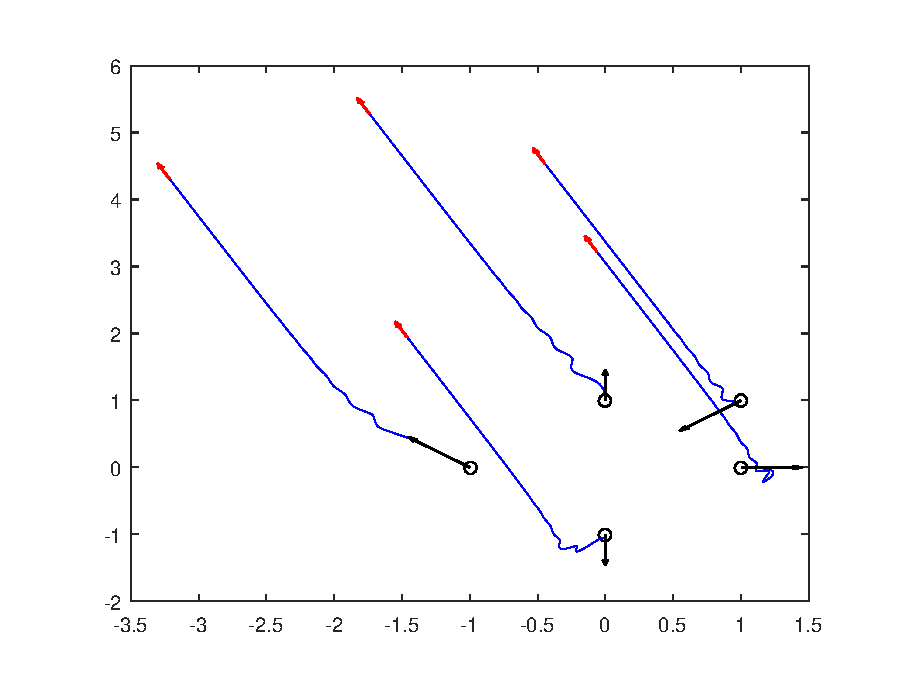
\includegraphics[width=\textwidth]{figures/a5_D_ev.eps}
    \caption{Evolution of the system}
    \label{ev}
  \end{minipage}
  \hfill
  \begin{minipage}[b]{0.5\textwidth}
    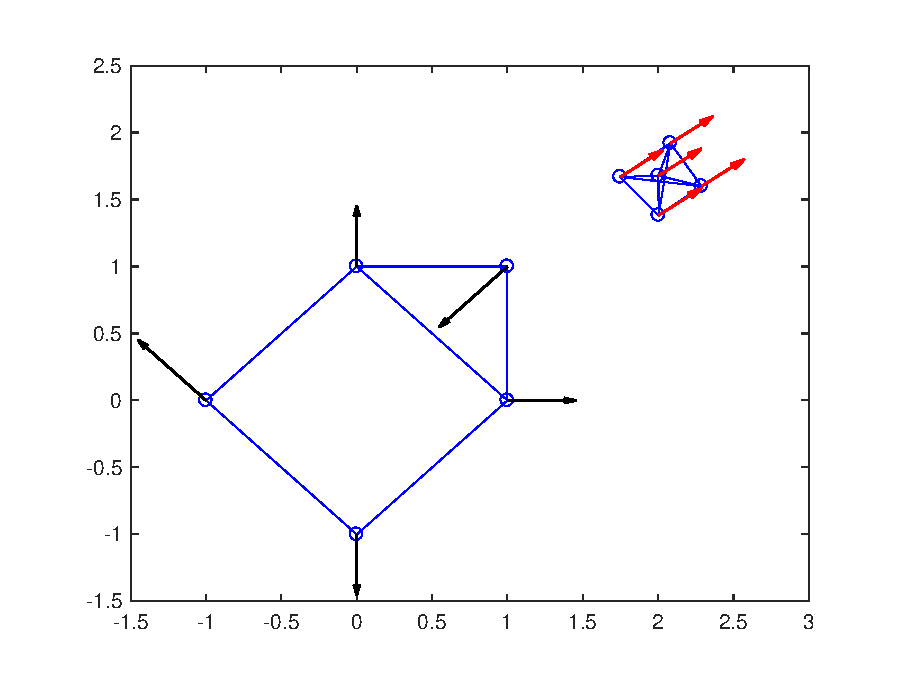
\includegraphics[width=\textwidth]{figures/a5_D_g.eps}
    \caption{Initial and terminal configurations}
    \label{g}
  \end{minipage}
\end{figure}

\begin{figure}[ht]
  \begin{minipage}[b]{0.5\textwidth}
    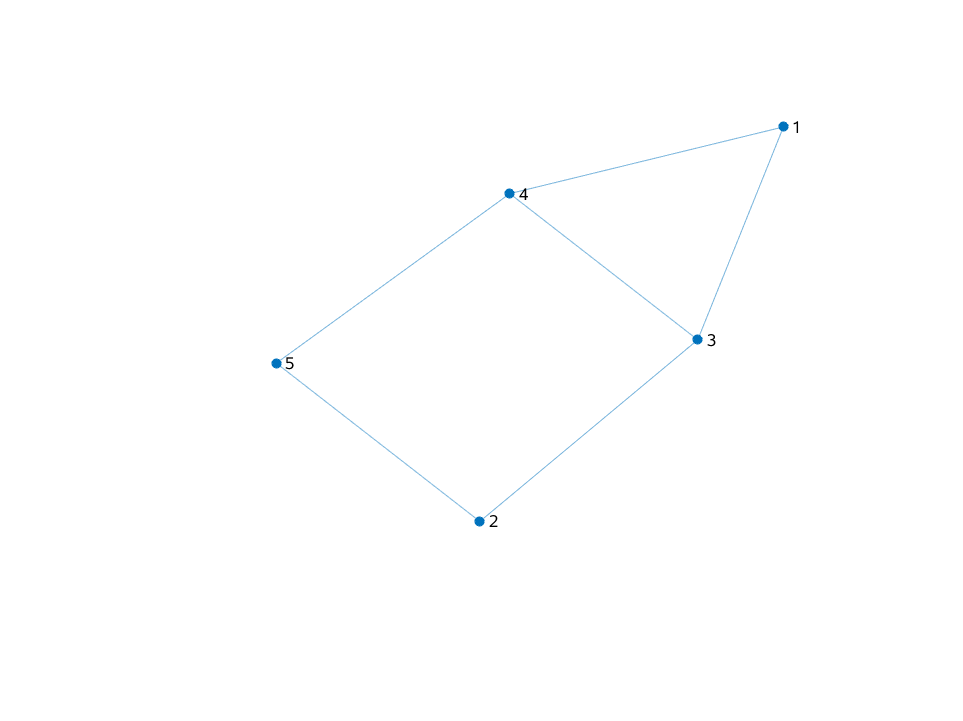
\includegraphics[width=\textwidth]{figures/a5_D_cg0.eps}
    \caption{Connectivity at the initial configuration}
    \label{g0}
  \end{minipage}
  \hfill
  \begin{minipage}[b]{0.5\textwidth}
    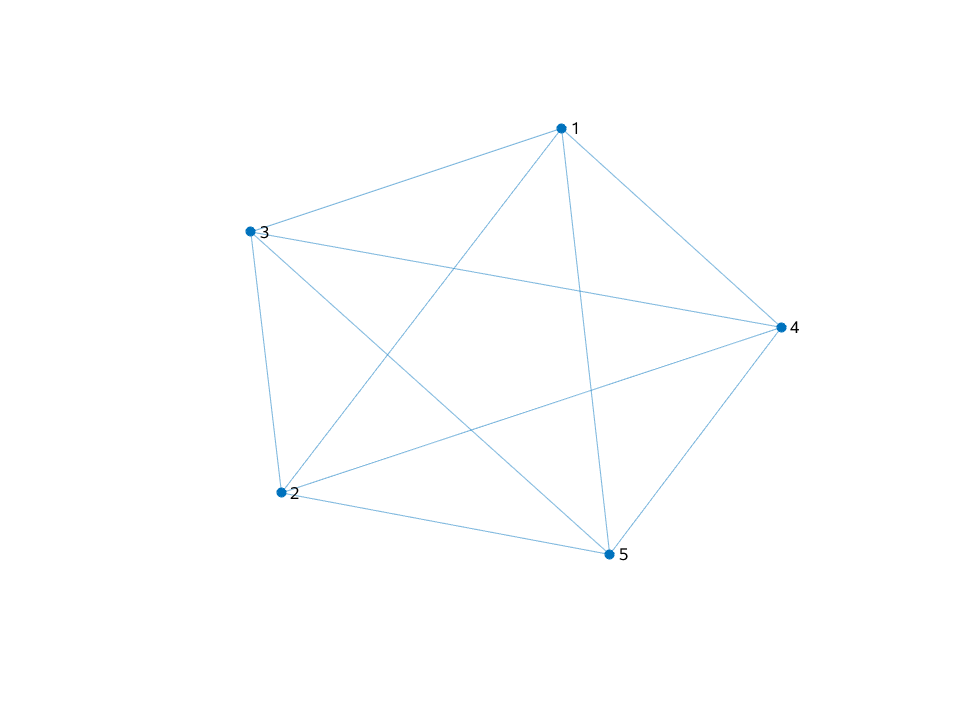
\includegraphics[width=\textwidth]{figures/a5_D_cgT.eps}
    \caption{Connectivity at the terminal configuration}
    \label{gT}
  \end{minipage}
\end{figure}
  
 
 \begin{figure}[ht]
 \centering
 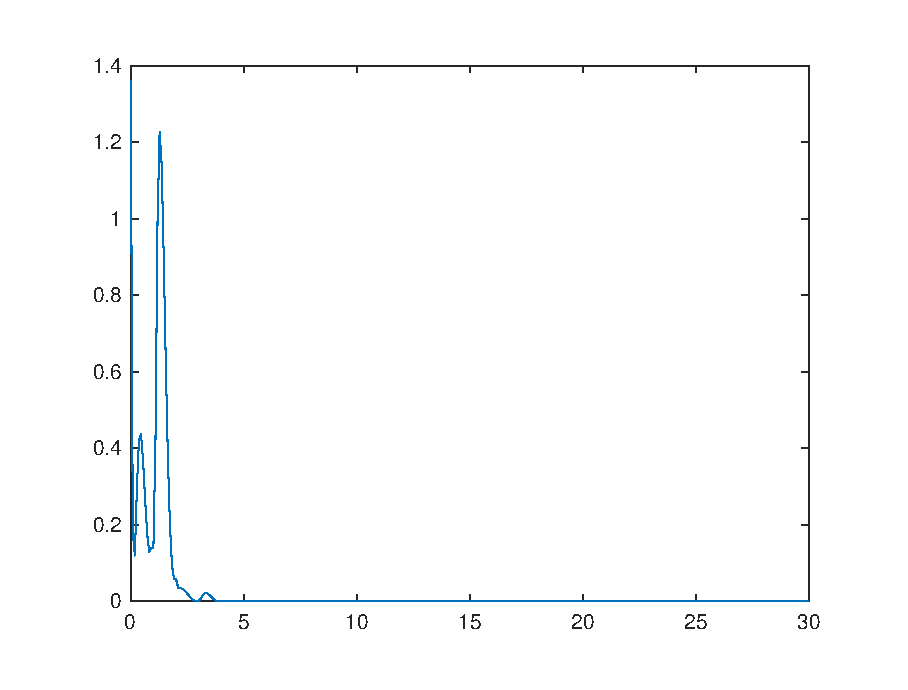
\includegraphics[scale=0.5]{figures/a5_D_lf.eps}
 \caption{$B(v(t), v(t))$}
 \label{lf}
 \end{figure}
  \newpage
The evolution of the system can be observed on the Figure \ref{ev}. On the Figure \ref{lf} we see the velocity deviation throughout the evolution. The bump in the velocity deviation $B(v(t), v(t))$
is due to the fact that initially the control steers the agents towards each other and after the completeness of the network graph (see Figure \ref{gT}) is reached it brings smoothly the system to consensus with terminal value of velocity deviation $B(v^{mn}, v^{mn})$ tends to zero. Under such terminal configuration the system has entered the consensus region in time  $t^* = 1.823$ since  $E(x(t), v(t)) < 0$ for all $t>t^{*}$ and the system tends to consensus uncontrolled.

We also consider the centralized optimal control strategy (\ref{j}) - (\ref{csm}) for the same configuration. The evolution of the system controlled by centralized strategy (\ref{j}) -(\ref{csm}) can be observed on Figure \ref{evc}, as in the previous example the black arrows denote initial velocities and the red ones velocities in the terminal configuration.  The terminal values 
of velocity deviation $B(v^{mn}, v^{mn})$ tends to zero and the consensus quantity (\ref{cq}) becomes negative after time $t^* = 0.825$,  $E(x(t), v(t)) < 0$ for all $t>t^{*}$. On Figure \ref{lfc} the evolution of velocity deviation is present.
\begin{figure}[ht]
  \begin{minipage}[b]{0.5\textwidth}
    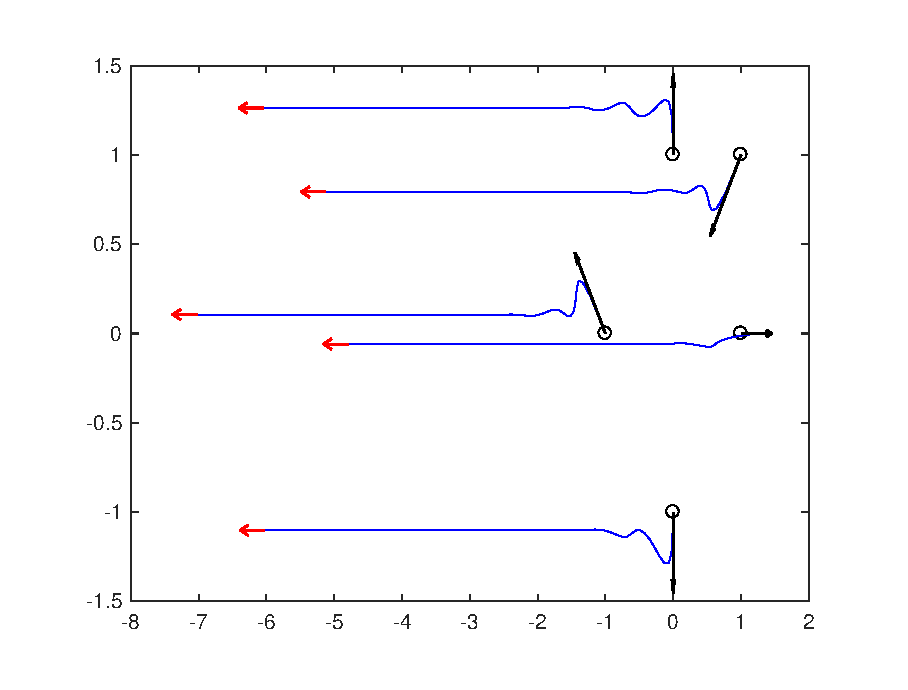
\includegraphics[width=\textwidth]{figures/a5_C_ev.eps}
    \caption{Evolution of the system}
    \label{evc}
  \end{minipage}
  \hfill
  \begin{minipage}[b]{0.5\textwidth}
    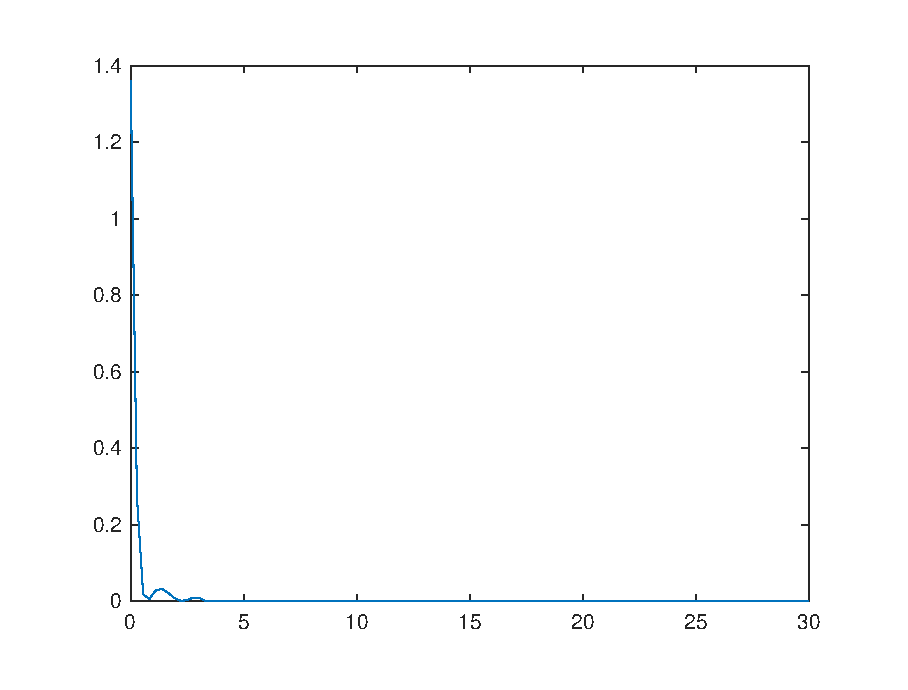
\includegraphics[width=\textwidth]{figures/a5_C_lf.eps}
    \caption{$B(v(t), v(t))$ }
    \label{lfc}
  \end{minipage}
\end{figure}

Here we compare the norm of controls for both centralized and decentralized control strategies. 
\begin{figure}[ht]
  \begin{minipage}[b]{0.5\textwidth}
    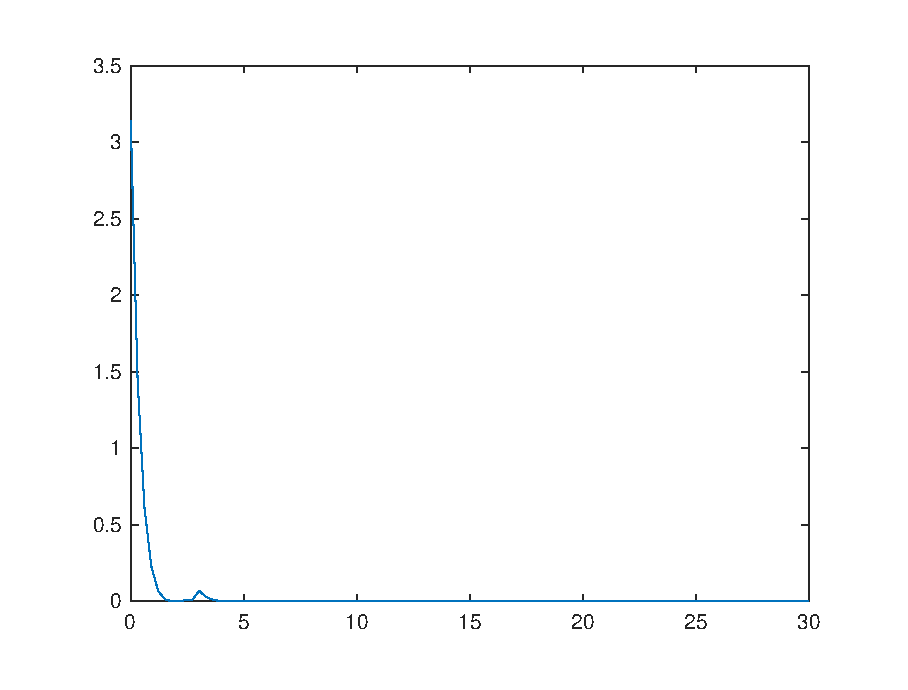
\includegraphics[width=\textwidth]{figures/a5_C_c.eps}
    \caption{Centralized control energy}
    \label{cc}
  \end{minipage}
  \hfill
  \begin{minipage}[b]{0.5\textwidth}
    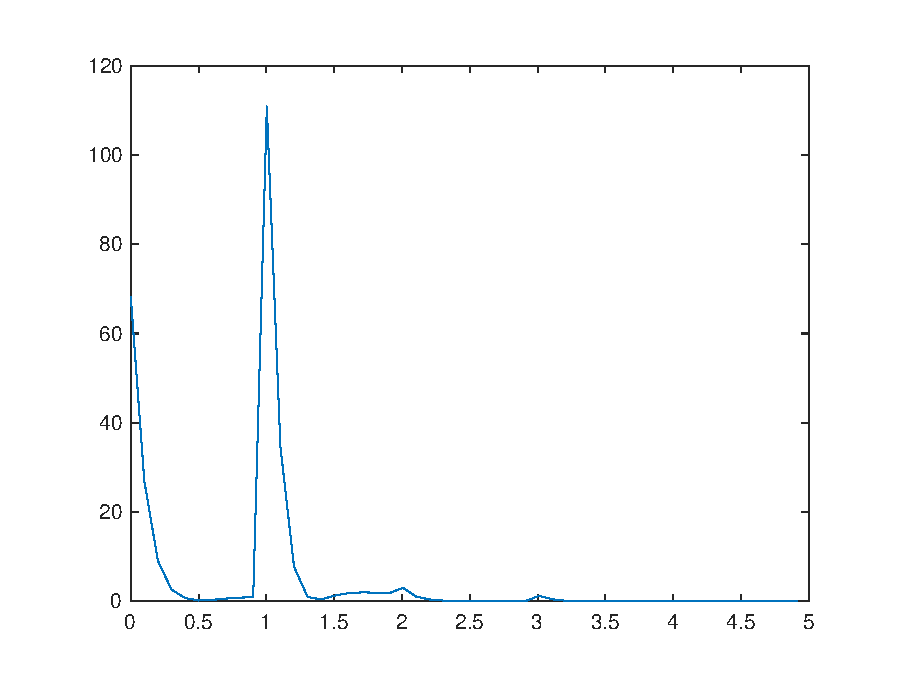
\includegraphics[width=\textwidth]{figures/a5_D_c.eps}
    \caption{Decentralized control energy}
    \label{dc}
  \end{minipage}
\end{figure}2

In our experiments the decentralized control turns to be more expensive, what apparently is the cost which comes with the decentralization. 
The energy to control the system spend by centralized control in Figure \ref{cc} amounts to  $\int_{0}^{T} \|u^c(t)\|_2 dt  = 1.56$, whereas that of decentralized on Figure \ref{dc} $\int_{0}^{T} \|u^d(t)\|_2 dt  = 28.27$.


 The connection radius is $R = 2$. 

 \section{Example 2}
  Here we compare the decentralized heuristic feedback control (\ref{myhc}) with control (\ref{controljad}).
System (\ref{csm}) controlled by (\ref{myhc}) tends to consensus almost instantly preserving the connectivity of the network. The consensus region is reached 
  in time   $t^* = 0.062$ since  $E(x(t), v(t)) < 0$ for all $t>t^{*}$, whereas the control (\ref{controljad}) steers the system to consensus region in considerably larger time  $t^* = 1.089$.
  The evolution of systems (\ref{csm}), (\ref{myhc}) and (\ref{csm}), (\ref{controljad}) is present on Figures \ref{my_h_ev} - \ref{jad_h_ev} respectively.
  The support of velocity deviation throughout the evolution of both systems is demonstrated on Figure \ref{both_h_lf}, where we can observe that velocity alignment of the (\ref{myhc}) controlled system is much faster and more rapid.
  \begin{figure}[ht]
    \begin{minipage}[b]{0.5\textwidth}
      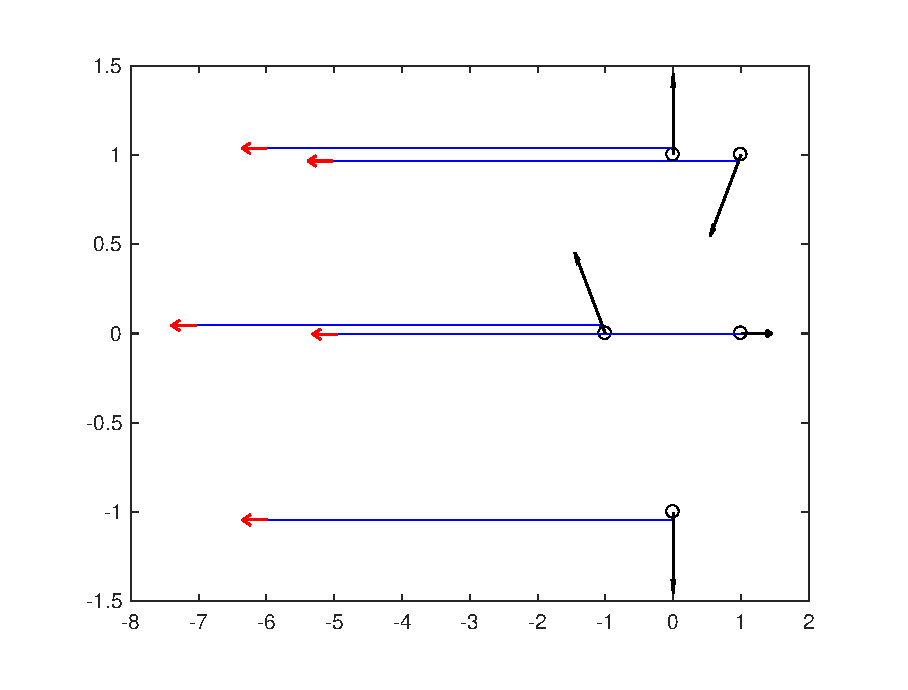
\includegraphics[width=\textwidth]{figures/my_h_ev.eps}
      \caption{Evolution of the system controlled by (\ref{myhc})}
      \label{my_h_ev}
    \end{minipage}
    \hfill
    \begin{minipage}[b]{0.5\textwidth}
      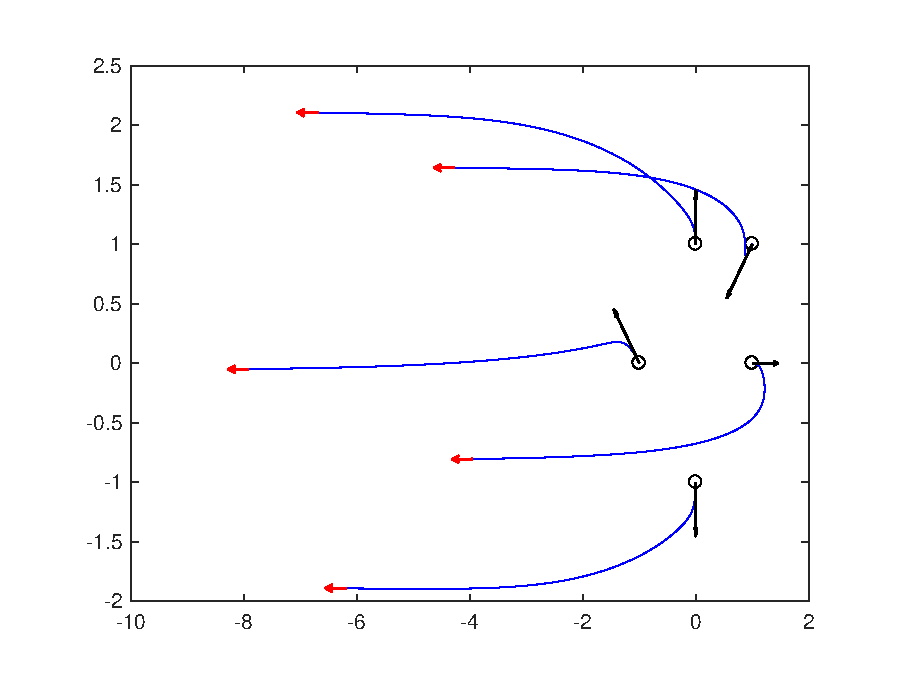
\includegraphics[width=\textwidth]{figures/jad_h_ev.eps}
      \caption{Evolution of the system controlled by (\ref{controljad})}
      \label{jad_h_ev}
    \end{minipage}
  \end{figure}
  
   \begin{figure}[ht]
   \centering
   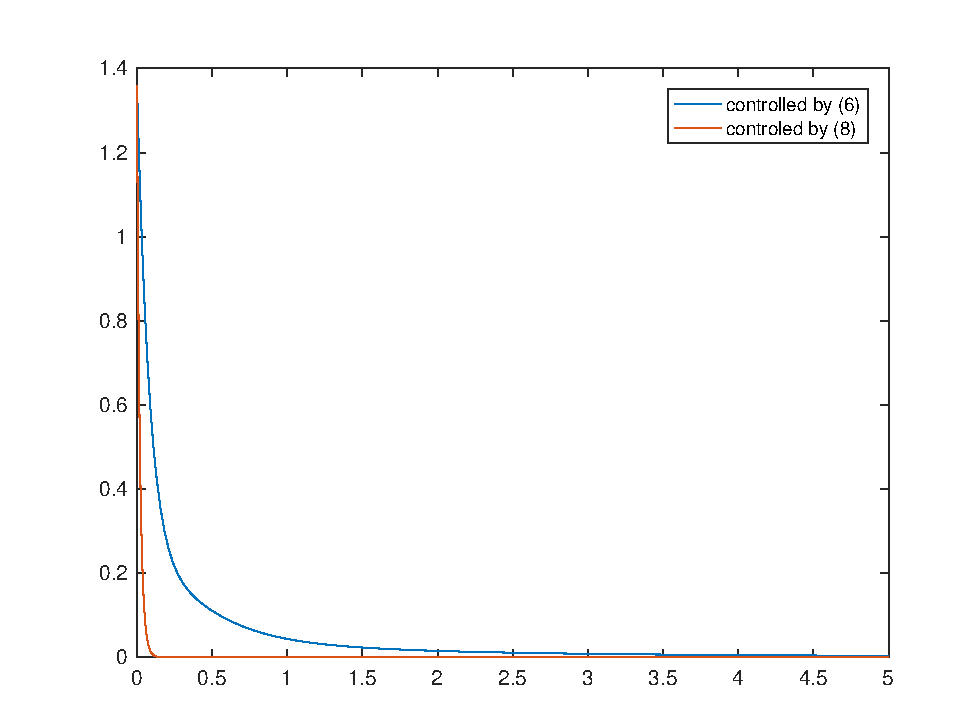
\includegraphics[scale=0.5]{figures/both_h_lf.eps}
   \caption{$B(v(t), v(t))$}
   \label{both_h_lf}
   \end{figure}
  
  
  
  \bibliography{mybib}{}
  \bibliographystyle{plain}
  
\end{document}
